\begin{voorstel}{Waterstof}
\meeschrijver{Mark Leenen}

\headerimg{img/energie/waterstof-header}
% https://commons.wikimedia.org/wiki/File:Berkhof_Ambassador_op_waterstof.jpg
% TODO: zijn we wel fan van waterstofbussen?

\begin{samenvatting}
In 2030 wordt groene waterstof gebruikt als energiebron als aanvulling op duurzamere en efficiëntere energiebronnen, zoals zon- en windenergie. Door de ontwikkeling van een waterstofeconomie worden veel banen gecreëerd. Wereldwijd is Nederland koploper in waterstoftechnologie.
\end{samenvatting}

\begin{multicols*}{2}

\begin{uitdaging}
Waterstof is een gas dat gebruikt kan worden als opslagmiddel voor energie (elektriciteit), of als brandstof voor industriële processen op hoge temperatuur, of als grondstof voor de (chemische) industrie. Via brandstofcellen kan waterstof omgezet worden in elektriciteit, bijvoorbeeld voor de aandrijving van elektromotoren in de transportsector. 
Er wordt onderscheid gemaakt tussen grijze, blauwe en groene waterstof. Waterstof wordt momenteel vooral gemaakt uit koolwaterstoffen zoals aardgas. Dit wordt grijze waterstof genoemd, omdat er  CO2 vrijkomt. Wanneer de vrijgekomen CO2 wordt opgeslagen, wordt gesproken van blauwe waterstof. Door met elektriciteit watermoleculen te splitsen, kan waterstof ook worden geproduceerd zonder CO2 uitstoot. Dit is groene waterstof. Idealiter is de elektriciteit die wordt gebruikt duurzaam opgewekt. Vaak worden groene waterstof en windmolenparken op zee in 1 adem genoemd.

Nederland is momenteel na Duitsland al de grootste producent van waterstof in Europa, met een productie van 8 miljard m3 per jaar. Deze (grijze) waterstof is vooral bedoeld als grondstof voor de chemische industrie, en zal de transitie moeten maken via blauw, naar groen. Alle infrastructuur die geschikt is voor grijze of blauwe waterstof, is ook geschikt voor groene waterstof.

Groene waterstof is alleen rendabel bij voldoende schaalgrootte. Die schaalgrootte kan alleen ontstaan bij voldoende vraag. Vraag en aanbod moeten samen gestimuleerd worden om de waterstofeconomie van de grond te krijgen.

Waterstofgas heeft andere eigenschappen dan aardgas (methaan). Technische uitdagingen zitten in het geschikt maken van delen van het aardgasleidingnetwerk voor waterstof. En in de toepassing van waterstof als brandstof in hoog-temperatuur processen in de industrie.
\end{uitdaging}

\begin{overwegingen}

\includegraphics[width=.5\textwidth]{img/energie/waterstof-tank}

Waterstof is een energie-opslag medium. Het opslaan en vrijmaken van energie in waterstof kost ook energie. Qua energie-efficientie scoort waterstof geen hoge ogen en zal daarom alleen een rol spelen in decarbonisatie van processen en sectoren waar decarbonisatie op andere manieren (zoals directe elektrificering) niet mogelijk is. Gedurende de jaargetijden waarin zonnepanelen veel energie opwekken, en in tijden van veel wind(energie), kan het overschot opgeslagen worden in de vorm van waterstof. In de maanden waarin weinig zonne-energie opgewekt wordt, of wanneer het minder waait, wordt het tekort dan aangevuld vanuit waterstof.

Nederland is goed gepositioneerd om een leider te worden in de waterstofeconomie. De Noordzee biedt gelegenheid voor grote windparken, waarvan de duurzame elektriciteit gebruikt kan worden voor elektrolyse van water tot groene waterstof. Nederland heeft een bestaande gas-infrastructuur die deels geschikt gemaakt kan worden voor waterstof. En Nederland heeft een sterke logistieke en chemische sector, waar waterstof goed in zal passen. Daarnaast heeft Nederland grote lege gasvelden, waar CO2 in opgeslagen kan worden vanuit de productie van blauwe waterstof.

Windparken op zee zullen een belangrijke rol spelen in de waterstofproductie. Op zee kunnen electrolyzers worden aangedreven met de opgewekte elketriciteit om waterstof te maken. In het verlengde daarvan kan transport van waterstofgas, boven transport van electriciteit, een kostprijsvoordeel opleveren [hy-gro].

Waterstof kan een belangrijke rol gaan spelen in internationaal vrachtverkeer. Deze sector heeft zich verenigd in de European Clean Trucking Alliance (ECTA). Al vanaf 2021 kan de Total Cost of Ownership van een vrachtwagen die rijdt op waterstof, concurreren met diesel. Vanaf 2021 kan ook langzaam accijns geheven worden op waterstof, om de investeringen in de waterstofeconomie terug te gaan verdienen. Vrachtwagens die waterstof verbruiken kunnen mede door Nederlandse bedrijven ontwikkeld en gebouwd worden (DAF en Scania, Holthausen Clean Technology). Ook in de scheepvaart wordt de toepassing van waterstof onderzocht, zoals in het Blue Dolphin project. [Hydrogen4climateaction.eu]

De lancering van de European Clean Hydrogen Alliance (ECH2A) op 8 juli 2020 laat zien dat Europa vol op waterstof in wil zetten. In Hydrogen Europe is de complete productieketen voor waterstof vertegenwoordigd door 160+ bedrijven, inclusief Nederlandse spelers. Ook lopen er al projecten om groene waterstof van en naar Nederland te transporteren (Green Spider, Green Flamingo \& H2Go, hydrogen4climateaction.eu).

In de industrie zal waterstof een rol spelen als brandstof voor industriële processen die een temperatuur > 250 C nodig hebben [Quintel]. Die processen zijn namelijk moeilijk direct te electrificeren. Momenteel wordt waterstof al bijgemengd bij methaan voor zulke processen. Ook kan waterstof op termijn biomassa vervangen als brandstof. Waterstof kan ook in plaats van methaan als grondstof dienen voor productie van kunstmest, en toepassing in de staalindustrie biedt eveneens mogelijkheden tot decarbonisatie.

Het huidige gasnet wordt aangepast en uitgebreid, zodat het in 2030 ook deels gebruikt kan worden voor transport van waterstof. Die waterstof is echter vrijwel niet bestemd voor huishoudens, maar grotendeels voor de industrie en het transport. In de gebouwde omgeving is een zo klein mogelijke rol voorzien voor waterstof. Hier blijft “gasvrij” het credo, tenzij dat niet kan en een CV ketel op waterstof de beste oplossing blijkt (zoals voor oudere woningen die niet op een warmtepomp over kunnen vanwege slechte isolatie). Waterstof moet zoveel mogelijk worden getransporteerd via pijpleidingen en niet via trucks. Voor afstanden < 1000 km is de efficiëntie van transport van waterstof door pijpleidingen zeer goed (>95\%). [BOSSEL]

\end{overwegingen}

\begin{aanbevelingen}
De windparken op zee moeten in de toekomst een mix van elektriciteit en groene waterstof (middels electrolysers op zee) leveren.
Er moet een landelijk waterstof pijpleiding netwerk gerealiseerd worden waarop alle grote afnemers (industrie, transport) aangesloten worden. Het bestaande gasnet dient hiervoor als basis.

Zwaar transport (vrachtvervoer) stapt over op waterstof als brandstof, met toegewijde waterstoftankstations langs snelwegen, die aangesloten zijn aan het waterstof gasnet. Voor inclusie van internationaal transport is het onontbeerlijk om de waterstofeconomie op Europees niveau te ontwikkelen. Particulier, lokaal en streekvervoer maakt in beginsel geen gebruik van waterstof als energiedrager, maar rijdt op batterijen.

Waterstof wordt gebruikt als brandstof in hoog-temperatuur processen in de industrie. Eerst zal blauwe waterstof worden gebruikt als geschikte tussenoplossing. Blauwe waterstof wordt lokaal geproduceerd en opgeslagen. Wanneer mogelijk wordt de overstap naar groene waterstof gemaakt. In de loop van de komende decade kan groene waterstof al bijgemengd worden bij blauwe of grijze waterstof, om vraag voor groene waterstof te creëren.

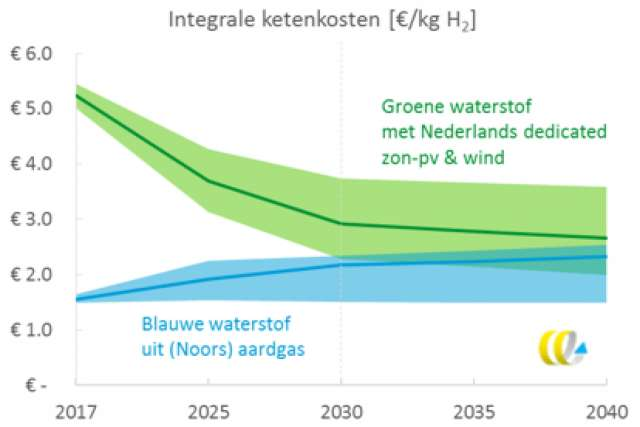
\includegraphics[width=.5\textwidth]{img/energie/waterstof-ketenkosten}

\end{aanbevelingen}

\paragraph{Literatuur}
http://hydrogeneurope.eu

http://hy-gro.net

Wind-to-hydrogen (W2H2) TKI Systeemintegratie Studie TES1216101

https://www.flightglobal.com/air-transport/forget-batteries-is-hydrogen-the-holy-grail-for-carbon-free-commercial-aviation/139150.article

\url{https://www.nrc.nl/nieuws/2020/07/08/brussel-omarmt-waterstof-a4005372#/handelsblad/2020/07/09/#301}

Ulf Bossel, “Does a hydrogen economy make sense?”, Proceedings of the IEEE, Vol. 94, No. 10, 2006, 1826 - 1837

J. Reijerkerk and G. van Rhee, “Waterstof: kansen voor de Nederlandse industrie”, Oktober 2019

https://clean-trucking.eu/publications/europes-opportunity-to-decarbonise-the-road-freight-sector/

http://www.hydrogen4climateaction.eu

Commissie Economische Zaken en Klimaat, “Kabinetsvisie Waterstof en Routekaart Groen Gas: Position Papers Reader”, 7 mei 2020

Institute for Sustainable Process Technology, “Hychain 1,2 \& 3: Energy carriers and hydrogen supply chain”, december 2019

https://www.portofrotterdam.com/nl/havenkrant/havenkrant-43/grootste-groene-waterstoffabriek-van-europa

https://www.natuurenmilieu.nl/themas/energie/projecten-energie/waterstof/waterstof-de-waterstofladder/

\end{multicols*}

\end{voorstel}
